\documentclass{scrreprt}
\usepackage[french]{babel}
\usepackage[utf8]{inputenc}
\usepackage[usenames,dvipsnames]{color}
\usepackage{listings}
\usepackage{underscore}
\usepackage[bookmarks=true]{hyperref}
\usepackage{graphicx}
\DeclareGraphicsExtensions{.pdf,.png,.jpg}
\lstset{language=xml,frame=single, breaklines=true, basicstyle=\ttfamily,backgroundcolor=\color{white},basicstyle=\scriptsize, keywordstyle=\color{blue}, commentstyle=\color{Gray}, stringstyle=\color{red}, identifierstyle=\color{green}}

%%%% debut macro %%%%
\newenvironment{changemargin}[2]{\begin{list}{}{%
\setlength{\topsep}{0pt}%
\setlength{\leftmargin}{0pt}%
\setlength{\rightmargin}{0pt}%
\setlength{\listparindent}{\parindent}%
\setlength{\itemindent}{\parindent}%
\setlength{\parsep}{0pt plus 1pt}%
\addtolength{\leftmargin}{#1}%
\addtolength{\rightmargin}{#2}%
}\item }{\end{list}}
%%%% fin macro %%%%

\hypersetup{
    bookmarks=false, % show bookmarks bar?
    pdftitle={Projet SASIAE}, % title
    pdfauthor={Raynal Jean-Raymond, Dauphin Loïc, Clément Lansmarie, Hugo Brunie, Nicolas Belin, Benoit Gilbert, Théotime Méralli-Ballou}, % author
    pdfsubject={TeX and LaTeX}, % subject of the document
    pdfkeywords={TeX, LaTeX, graphics, images}, % list of keywords
    colorlinks=true, % false: boxed links; true: colored links
    linkcolor=blue, % color of internal links
    citecolor=black, % color of links to bibliography
    filecolor=black, % color of file links
    urlcolor=purple, % color of external links
    linktoc=page % only page is linked
}%1 
\def\myversion{}
\title{
\flushright
\rule{16cm}{5pt}
\vskip1cm
{\Huge Rapport de PFA - Projet SASIAE}\\
\vspace{9cm}
{\small Théotime Méralli-Ballou\\ Jean-Raymond Raynal\\ Clément Lansmarie\\ Benoit Gilbert\\ Loïc Dauphin\\ Nicolas Belin\\ Hugo Brunie\\ }
\vfill
{\small Client: Aymeric Vincent / EIRBOT }
\rule{16cm}{5pt}
}
\date{}
\usepackage{hyperref}

\begin{document}

\maketitle
\tableofcontents

\chapter{Introduction}
Ce document présente le travail effectué dans le cadre du projet de deuxième année (PFA) de l'ENSEIRB-MATMECA qui avait pour objectif la création d'un simulateur pour robots.
Il opposera le cahier des charges et les choix de conception au produit finalement obtenu. Cela permettra de mettre en évidence les difficultés rencontrées lors du développement du projet, les choix et concessions qu'il a fallu faire au cours des derniers mois. Chacune de ces difficultés a permis aux membres de l'équipe d'acquérir de nouvelles compétences.

\section{Le contexte}

Le cadre de ce projet de PFA était peu commun puisqu'il a été soumis et réalisé par des élèves de l'école. Il s'agit de l'association de robotique de l'école, EIRBOT. Le sujet a donc été proposé par l'association pour améliorer son potentiel lors de la Coupe de France de robotique. Elle rassemble chaque année près de 200 équipes. De nombreuses équipes s'appuient sur une expérience longue de plusieurs années et utilisent des logiciels de simulation et bibliothèques améliorés d'année en année. Ce projet a donc pour objectif de permettre à Eirbot de fiabiliser ses robots, de faciliter l'écriture du code de stratégie, et ainsi de progresser dans le classement. Néanmoins l'association ne pouvant être cliente du PFA (car représentée par des élèves de deuxième année), l'enseignant chercheur Aymeric Vincent a accepté de tenir le rôle du client.

\begin{figure}[!h]
\centering
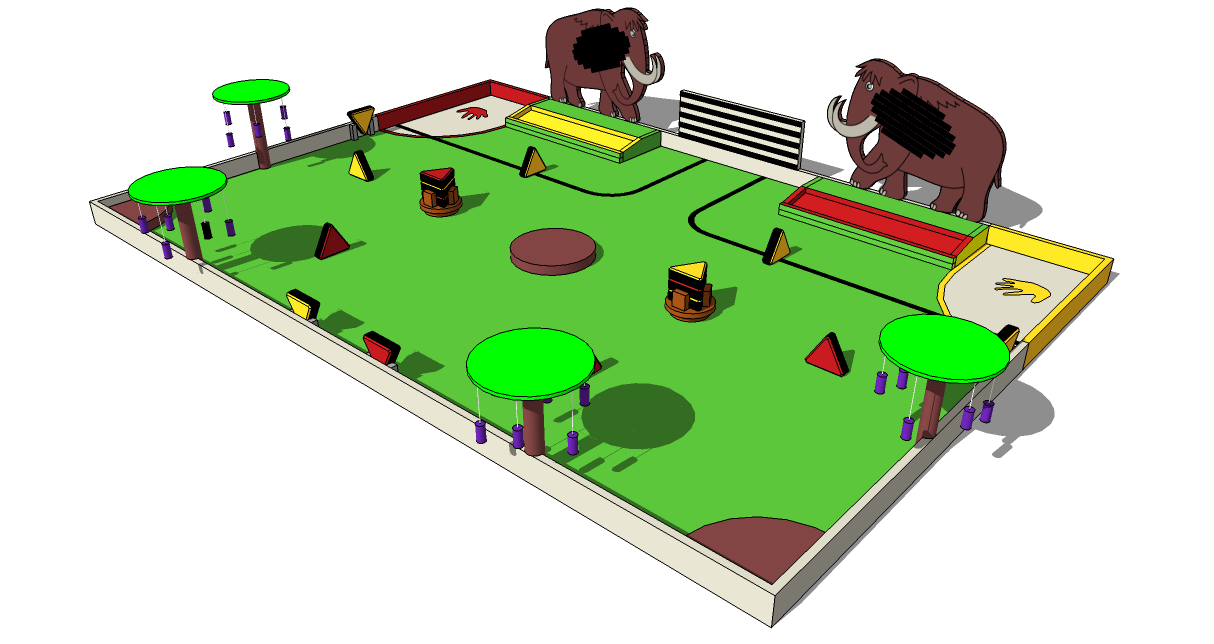
\includegraphics[scale=0.33]{table}
\caption{Table de jeu de l'édition 2014.}
\label{table}
\end{figure}

\paragraph{}
Afin d'avoir une meilleure idée de ce sur quoi s'appuie ce projet, nous proposons une rapide description du règlement de la coupe 2014 et du robot des deuxièmes années.

Comme chaque année, les robots doivent partir d'une zone délimitée de la table. À partir du top départ, ils disposent de 90 secondes pour marquer un maximum de points. Le moyen de faire des points diffère d'année en année. Cette année il est possible de :
\begin{itemize}
\item Récupérer les fruits pendus aux arbres en bord de table pour les verser dans le bac de sa couleur (au pied des mammouths)
\item Faire tomber les triangles, avec la couleur de son équipe face visible
\item Poser une "peinture" de sa couleur sur la fresque entre les deux mammouths
\item Lancer des balles de ping pong sur le velcro des mammouths
\item Lancer un filet au dessus d'un mammouth
\end{itemize}
En plus de marquer des points, le robot doit pouvoir éviter les robots adverses, ou au moins s'arrêter. À la fin des 90 secondes, les robots s'arrêtent et les arbitres procèdent au décompte des points.

\begin{figure}[!h]
\centering

\includegraphics[scale=0.1]{robot}
\caption{Aperçue du robot des deuxièmes années.}
\label{robot}
\end{figure}

\paragraph{}
Le robot n'est pas encore terminé, mais son fonctionnement actuel est quasiment final. Sa stratégie sera basée sur un déplacement précis qui permettra de récupérer les fruits, les mettre dans le bac correspondant, placer les peintures sur la fresque, et lancer les balles sur les mammouths. En fin de match il essaiera de lancer le filet sur un mammouth. Pendant les matchs, il essaiera également de faire tomber des triangles du bon côté mais cela pourra largement varier en fonction de l'efficacité des robots adverses.

\begin{figure}[!h]
\centering
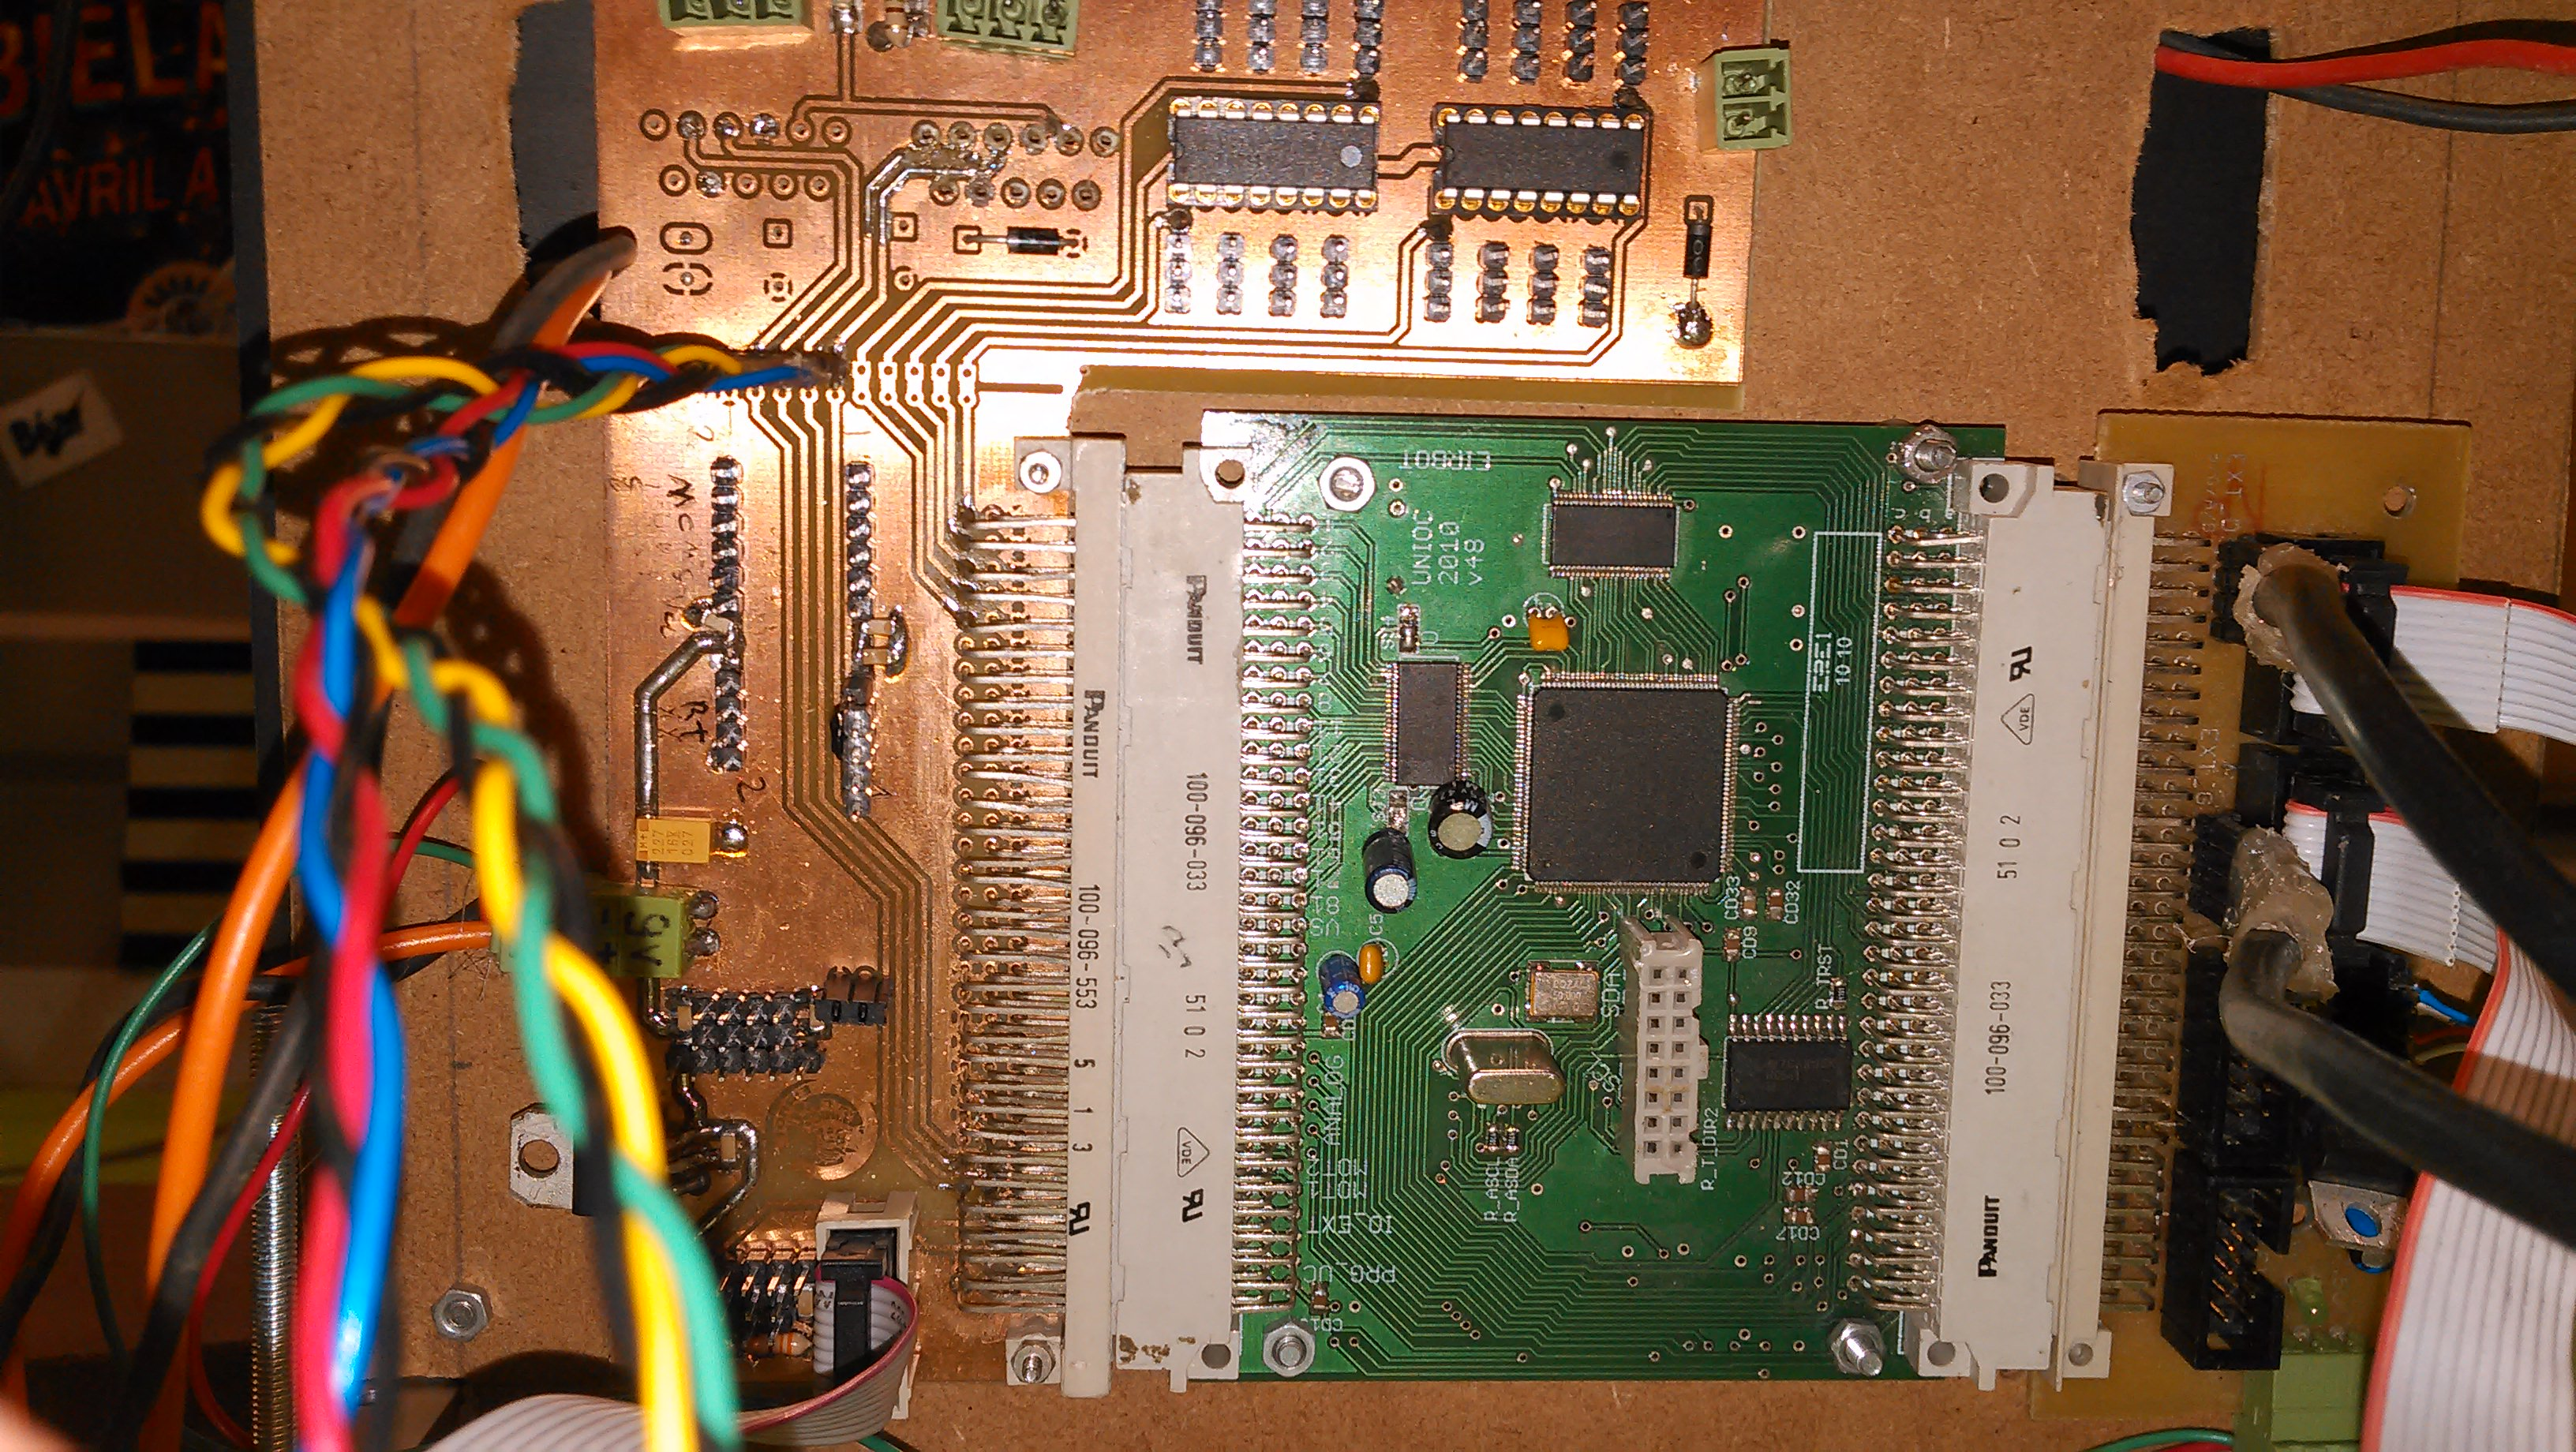
\includegraphics[scale=0.1]{unioc}
\caption{UNIOC : principale carte du robot.}
\label{unioc}
\end{figure}

\paragraph{}
La carte électronique principale du robot \ref{unioc} est appelée carte UNIOC. Cette carte contient toute la stratégie du robot, gère le déplacement, l'évitement d'éventuels adversaires. Elle dispose de l'essentiel de la puissance de calcul du robot. Jusqu'à présent, elle utilisait le framework Aversive, écrit par d'anciens élèves de l'école (expliqué ci-dessous). Cette carte envoie les commandes à tous les moteurs et actionneurs du robot. Elle communique également avec d'autres cartes telles que celle de détection d'adversaire \ref{rds} pour ajuster sa stratégie en fonction de la position des autres robots.

\begin{figure}[!h]
\centering
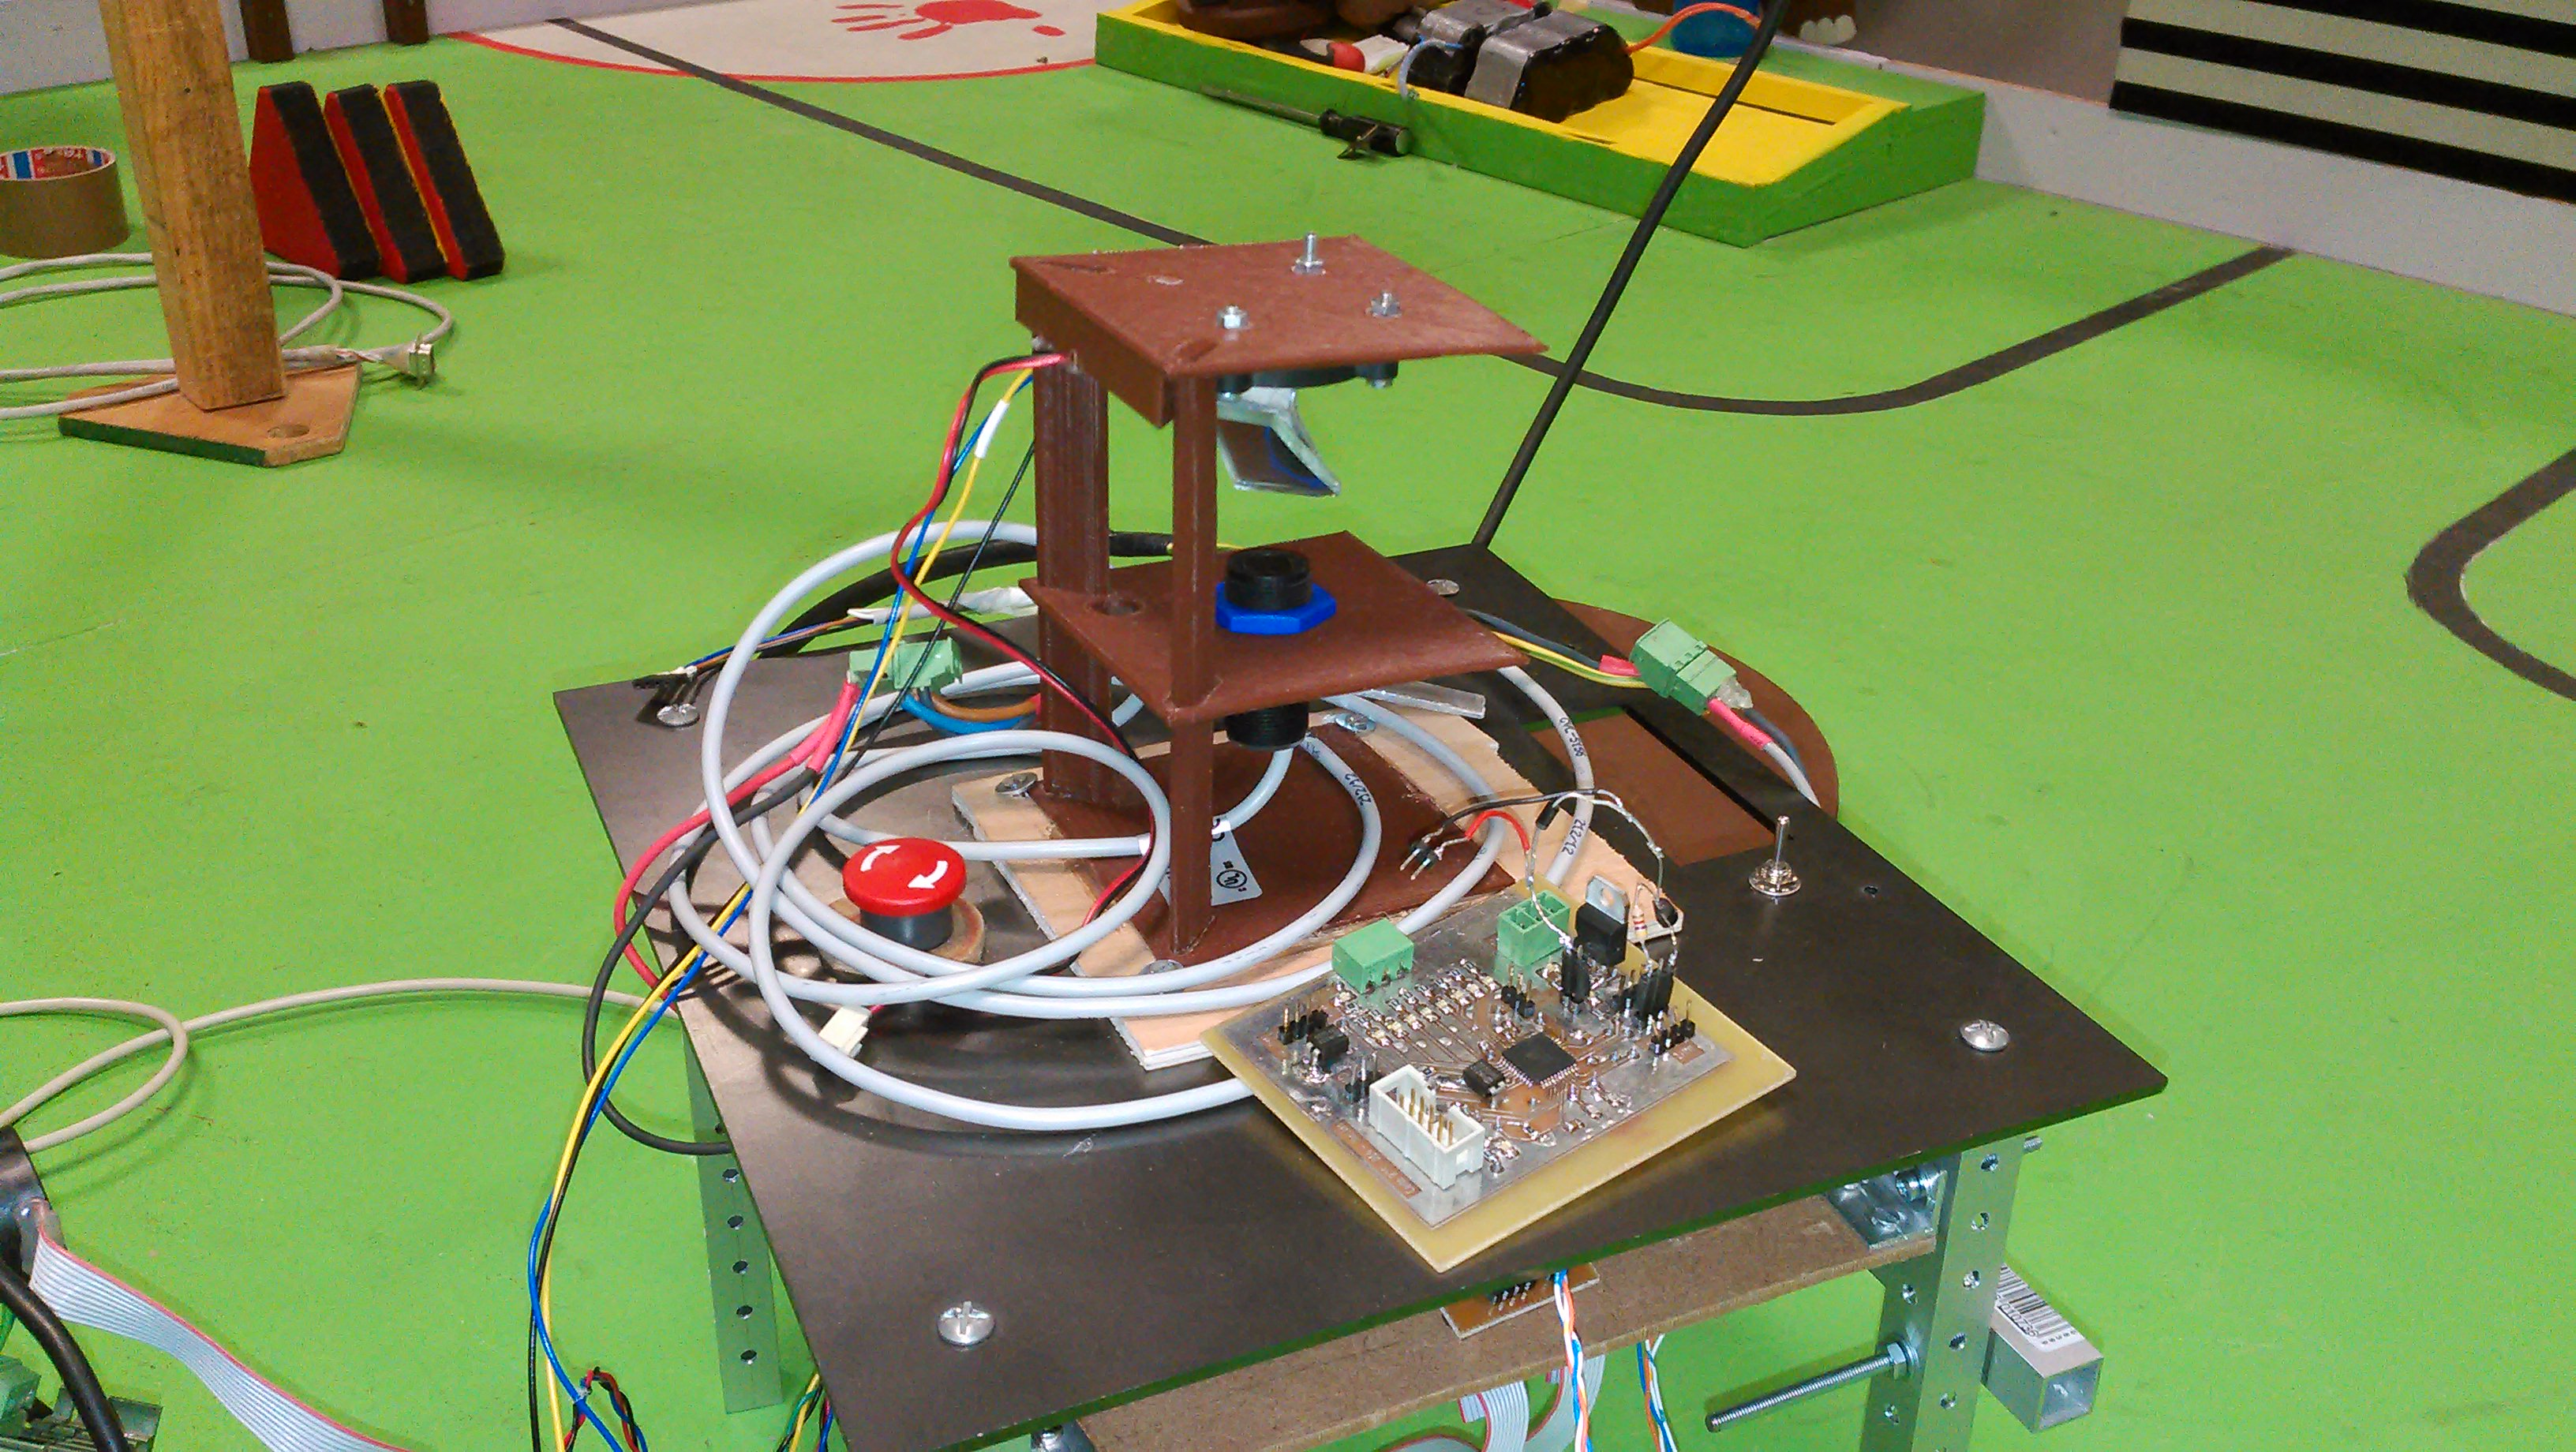
\includegraphics[scale=0.1]{rds}
\caption{Système de détection de robots adverses.}
\label{rds}
\end{figure}

\section{Objectifs}

Le résultat souhaité par le client EIRBOT est un simulateur de robot. Ce simulateur doit afficher le déplacement d'un ou plusieurs robot sur la table vue de dessus, en temps réel. Il prend en entrée un code robot et une description du robot et de la table. Un robot doit pouvoir interagir avec son environnement grâce à ses capteurs. Le simulateur doit donc être en mesure de calculer les valeurs à renvoyer aux capteurs du robot en fonction de s'il rencontre un obstacle, un autre robot, etc...

Cette spécification est primordiale pour le client, car le principal objectif du simulateur est d'afficher un déplacement du robot le plus proche possible de la réalité.
En effet, pour obtenir un bon score à la coupe de France de robotique à laquelle participe Eirbot, il est important de maîtriser son déplacement sur la table. Un déplacement "intelligent" comprend un évitement efficace des obstacles et des robots adverses, et il s'agit d'une des priorités pour l'équipe Eirbot.

\paragraph{}
Ce projet contient également, en partie, la réécriture du framework (Aversive) qui existe déjà à Eirbot et qui avait été écrit il y a 7 ans par des élèves de l'école. Ce framework gère les interruptions, propose des primitives de haut niveau pour déplacer le robot sur la table, et des interfaces de communication avec les entrées et sorties.

Le besoin de réécrire Aversive est dû au fait qu'au fil des ans, la compréhension de cet outil se perd et qu'il est de plus en plus difficile pour les nouvelles années de le débugguer ou de l'exploiter à son plein potentiel.
EIRBOT souhaite donc disposer d'un nouveau framework (Aversive++) mieux documenté. Cependant seule la réécriture de l'API d'Aversive++ est concernée par le projet SASIAE\footnote{Simulateur d'Asservissement de Stratégie et d'Intelligence Artificielle d'Eirbot}. 

Notre rôle a donc été la création de l'interface et le développement des fonctionnalités du nouveau framework destiné au simulateur, et l'association EIRBOT est en charge quant à elle de développer les mêmes fonctionnalités pour le microcontrôleur.

\paragraph{}
Le cahier des charges détaille les fonctionnalités souhaitées par EIRBOT pour le simulateur. De plus la majorité de l'équipe SASIAE étant également dans l'équipe Eirbot, ce qui n'aura pas été fait durant le PFA, notamment par manque de temps, sera implémenté plus tard par les membres d'Eirbot.

\paragraph{}
Le \textbf{S}imulateur d'\textbf{A}sservissement, de \textbf{S}tratégie et d'\textbf{I}ntelligence \textbf{A}rtificielle d'\textbf{E}IRBOT prenait ainsi vie, sous le nom plus élégant de SASIAE.



\chapter{Génie logiciel et management de projet}
\section{Gestion du projet}

Le PFA constitue le projet le plus important que nous ayons réalisé. L'organisation du projet, l'architecture logicielle, la gestion du temps, la répartition des tâches au sein de l'équipe et le découpage de notre équipe en sous-équipes sont autant d'éléments qui ont pris une toute nouvelle envergure pour nous.

\section{Découpage du temps}

Nous avions découpé dans le cahier des charges le projet en plusieurs livrables, allant de la version minimaliste attendue par le client à la version optimale. Le planning a été construit autour de ces cinq livrables de telle sorte que soit réduit le risque de se retrouver sans simulateur utilisable à la fin du projet. Toutes les trois semaines en moyenne un livrable devait être fini pour nous permettre de passer au suivant.
Sur les cinq livrables prévus, nous n'avons pu aller plus loin que le 4ème livrable, mais celui-ci n'en reste pas moins exploitable par le client EIRBOT.

Le planning n'a pas tout à fait respecté les livrables tels quels en fonction de notre avancée. C'est à dire que certaines fonctionnalités ont été intégrées dans un livrable autre que celui prévu originalement, mais les modifications restent minimes. Cela est dû aux différentes difficultés que nous avons pu rencontrer sur des fonctionnalités qui finalement n'étaient pas vitales au projet.

\section{Méthode}

Nous avons principalement travaillé par groupes de deux ou trois pour les différentes tâches, avec des cycles d'environ deux semaines. Le planning de départ a été réparti entre les membres de l'équipe au hasard. Cela a permis à tout le monde de travailler sur tous les domaines abordés par le projet. Le principal problème de cette organisation a été le temps d'adaptation nécessaire à ces changements. De manière à structurer nos travaux nous avons essayé de mettre en place la méthode Kanban et de gérer les tâches en les triant entre les tâches à faire, faites et en cours de développement. Cela n'ayant pas fonctionné longtemps nous avons privilégiés des réunions hebdomadaires de l'équipe et des réunions avec notre encadrant pédagogique toutes les deux ou trois semaines.

\section{Stratégie de tests}

Ce projet a suivi la stratégie de test classique. Pour chaque objet nous avons implémenté des tests unitaires afin de vérifier le respect des spécifications et la correction des méthodes. Puis chaque partie a été intégrée petit à petit afin de vérifier leur bonne articulation et leur respect des attentes. Enfin, nous avons procédé à un test recette en simulant l'exécution d'un robot complet.
Le détail des test unitaires qui ont soulevé des problèmes pertinents est précisé dans la description détaillée du projet.
De plus l'annexe comporte une partie purement descriptive des tests à la section \ref{lestests}. 
L'écriture de test a été bénéfique, en effet la conception des classes et méthodes n'a pas toujours était optimale ou même correcte et les tests ont permis de mettre en évidence ces défauts.
Cependant, au fur et à mesure des itérations de notre méthode de développement certains tests sont devenus obsolètes parce qu'ils étaient liés à un état devenu obsolète de l'implémentation. 




\chapter{Description générale}
\section{Schéma global}

\begin{figure}[!h]
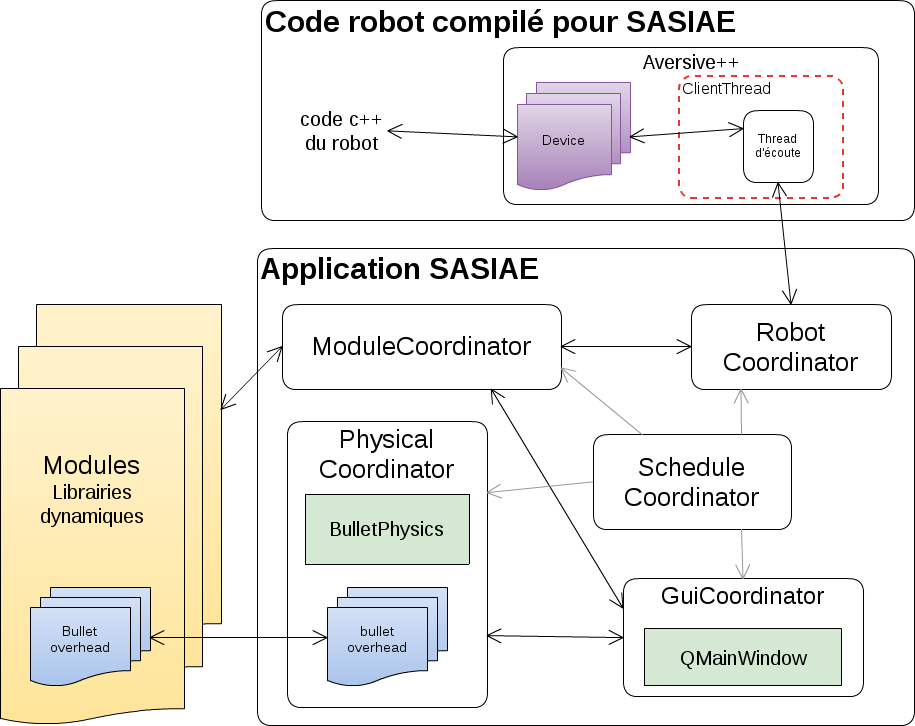
\includegraphics[width=\textwidth]{general}
\caption{Description générale du simulateur}
\label{descgenerale}
\end{figure}
\vspace{0 mm}
%\clearpage
L'architecture globale du projet est restée fidèle à celle du cahier des charges. Mais les difficultés rencontrées nous ont obligé à l'affiner quelque peu, comme par exemple l'éclatement du Coordinateur en plusieurs coordinateurs. Le détail des améliorations apportées sera effectué dans la section \ref{detail} et la figure \ref{descgenerale} reprend le schéma du cahier des charges enrichi des améliorations.

\section{Choix effectués}

\subsection{Contraintes de départ}

\paragraph{}
Il était prévu que plusieurs entités interagissent entre elles. Par conséquent nous voulions les abstraire le plus possible pour assurer l'indépendance des parties, le tout basé sur les conventions prises dans le cahier des charges. Pour ce faire, de nombreuses contraintes sont apparues dans l'écriture des classes intermédiaires. Ces contraintes de modularité et d'indépendance nous ont aussi amené à faire des choix que nous n'avions pas prévus dans le cahier des charges, comme par exemple la création d'une API pour le moteur de simulation physique. Celle-ci nous permet d'abstraire la communication avec Bullet.

De nombreuses semaines ont été nécessaires au lancement du projet pour pouvoir décider d'une architecture la plus cohérente possible. La taille du projet a fait que malgré toutes les précautions prises, il a fallu à quelques reprises revoir les choix que nous avions effectués.



%Du côté d'Aversive++, qui est le framework utilisé directement par le code robot, il a fallu abstraire la communication avec le reste du simulateur puisque les prototypes des classes et des méthodes employées est commun au simulateur et au robot. Il n'est donc pas question de lier ces classes au framework de Qt. Afin que tout puisse continuer à communiquer efficacement, malgré toutes les abstractions faites, il a fallu mettre l'accent sur le groupe des coordinateurs où chacun est dédié à la communication et synchronisation d'une partie spécifique du simulateur. 

\subsection{Programmation événementielle}

Pour rendre notre travail agréable à utilisé, il semble évident de faire une interface graphique. L'un des plus puissant framework libre actuel pour les réaliser est Qt. Or, ce framework nécessite de maîtriser un nouveau mode de programmation, la programmation événementielle. C'est un paradigme de programmation, à l'instar de la programmation séquentielle. Mais contrairement à cette dernière, au lieu de définir une séquence d'ordres donnés à la machine, la programmation événementielle consiste à définir comment l'application doit réagir lorsque tel ou tel événement se produit. Les événements auxquels peut réagir l'application sont nombreux et variés, allant de l'appui d'une touche au clavier, de la validation d'un formulaire ou d'un clic sur un bouton à un plus haut niveau mais aussi à l'arrivée d'un message réseau voire même l'envoi d'un message d'une entité interne à l'application. C'est dû à ce dernier point que la programmation événementielle est très souvent couplée avec l'orienté objet. En effet, les objets de l'application peuvent donc ainsi émettre des messages et d'autres objets qui écoutent ces messages réagiront en conséquence. De plus, la programmation événementielle permet une certaine aisance, facilitant la programmation d'interface graphique. En effet, pour la création d'interface graphique haut niveau, avec les outils adaptés, il suffit de placer les contrôles graphique de notre interface (menu déroulant, bouton, sélectionneur de couleur, etc) puis de définir le comportement de chacun des contrôles lorsqu'un événement utilisateur les concerne. Apprendre les mécanismes de cette méthode de programmation n'as pas été évident mais ce fut un réel enrichissement de notre culture technique. 


\section{Terminologie}
Nous allons aborder ici les quelques conventions utilisées par la suite. Tout d'abord, le projet comporte deux parties majeures qui sont l'API Aversive++ et le simulateur SASIAE, or ces deux entités possèdent théoriquement des implémentations de modules qui sont respectivement l'implémentation du code permettant d'exploiter un module et l'implémentation de l'image des actionneurs et des capteurs du Robot dans le simulateur. Les premiers seront donc nommés "device" par la suite tandis que les autres conservent le titre de "modules". De même, comme notre projet porte sur le monde de la robotique, le terme moteur physique portait à confusion. Nous appellerons donc calculateur physique les moteurs de calcul de la physique d'un environnement. Enfin, le projet nécessitait la mise en place d'un planificateur de tâches pour Aversive++ que nous avons nommé "Scheduler".






\chapter{Architecture détaillée}
\label{detail}

Dans cette section seront détaillés les différents aspects / entités qui interviennent dans le simulateur. Nous nous proposons pour chacune des parties de d'abord présenter le contexte de la partie en question, les choix faits dans le cahier des charges, puis de décrire les problèmes et difficultés rencontrées pour finalement opposer ce qui a été fait avec les choix de départ.

\section{Aversive++}

Bien que le développement d'Aversive++ pour microcontrôleur n'entrait pas dans le cadre du PFA, le support des microcontrôleurs AVR utilisés par le client EIRBOT n'en reste pas moins une contrainte forte sur le design de l'API. La deuxième contrainte principale étant son exploitation à des fins de simulations.

\paragraph{} %%\subsection{Choix de conception}

L'une des tâches principales du projet a donc été de ré-implémenter les devices avec lesquels l'association\footnote{EIRBOT est une association loi 1901} travaille. Le travail principal de ces derniers dans le cadre du simulateur étant de traiter les messages reçus de la simulations de manière à reproduire le comportement d'un robot lors d'une exécution de son code. Chaque device doit donc être identifié. Nous avions pensé à les identifier par leur nom dans le cas de ressources internes au microcontrôleur ou par leur pin (port sur lequel est connecté le device) s'ils étaient à l'extérieur du microcontrôleur. Afin de simplifier la communication entre le code robot et le simulateur, un device est systématiquement identifié par son nom. Dans tous les cas, cela a demandé une modification de l'API pour ajouter ce nom en paramètre aux constructeurs des devices (bien qu'utile uniquement à des fins de simulation). À premier abord, cela semble poser problème vis à vis des contraintes d'espace sur AVR. Néanmoins, nos constructeurs de devices étant en \texttt{inline} et le degré d'optimisation de la compilation étant important (\texttt{-O3}), le compilateur ne rajoute pas ces lignes si elles ne sont pas utilisées.

\paragraph{} %%\subsection{Difficultés rencontrées}

Développer Aversive++ a posé de nombreux problèmes, ceux-ci indiqués dans leurs parties respectives détaillées plus bas.

On peut citer néanmoins le type \texttt{SafeInteger} (permettant de faire des opérations arithmétiques \og sûres \fg) que nous n'utilisons finalement pas.

Le client avait demandé un moyen de détecter les erreurs d'overflow lors des calculs. Nous avions donc écrit une classe \texttt{SafeInteger} qui devait être utilisée en lieu et place des entiers classiques. Cependant lors d'une revue de cette classe, nous nous sommes rendus compte qu'elle n'était pas optimisée et ne fonctionnait pas correctement dans certaines situations critiques. Nous avons donc décidé de ne pas l'utiliser. En outre, son utilisation surchargeait les calculs.

\paragraph{} %%\subsection{Produit final}
Le cahier des charges prévoyait déjà un message de synchronisation mais uniquement pour ordonner au code robot de s'exécuter sur un pas de simulation. Ce message a été enrichi avec le temps écoulé depuis le début de la simulation pour permettre au planificateur de tâche de réaliser son travail. Une deuxième information est venu enrichir ce message de synchronisation, il s'agit d'un entier indiquant au code robot combien d'itérations de la boucle principale dans la fonction \texttt{main} il peut exécuter sur ce pas de simulation.

Parmi les contraintes de développement fixées dans le cahier des charges, la plupart on été respectées :

\begin{itemize}
\item utilisation des fonctions \texttt{inline} pour de petites fonctions pour assurer une optimisation du code à la compilation
\item utilisation de variables \texttt{const static} dès que possible
\item utilisation de \texttt{template} à la place de branchement conditionnel si possible de manière à rendre le code générique et plus rapide
\end{itemize}
Nous avions également pensé nous passer de l'utilisation de fonctions virtuelles afin d'alléger l'exécutable pour microcontrôlleur mais cela a posé d'importantes difficultés de conception lors de la création des devices. Cette contrainte est toute fois respectée dans la majorité du code.

\subsection{Client thread}

Aversive++ met à disposition de nombreux devices. Ces devices sont des interfaces haut niveau pour interagir avec du matériel. De ce fait, dans le cas de l'implémentation AVR, les devices apportent une surcouche par dessus les drivers. Hors, dans le cas de la simulation, le matériel n'est pas physiquement présent et il n'y a donc pas de driver non plus. La matériel a donc été représenté par des modules dans le simulateur. Or, ces modules se trouvent dans un processus différent que celui où s'exécutent le code robot et donc les devices. Nous avons donc mis en place un client dans Aversive++ (implémentation SASIAE) pour gérer la communication entre les devices et les modules (le protocole de communication étant détaillé plus loin).  Le client thread permet donc au device \og d'inscrire \fg\ leur nom avec une fonction qui traitera les messages qui leur seront destinés. Il permet également au device l'envoi de message au module ou l'envoi de message de Log. De plus, le \texttt{client thread} s'exécute dans un thread séparé du thread principale (d'où son nom) car il a besoin de continuer à recevoir et interpréter les messages qu'il reçoit, même lorsque le thread principale est bloqué, en attendant que la simulation avance. Une instance de device lui indique le traitement à réaliser lorsqu'il doit lui faire parvenir un message. Mettre en place une telle méthode n'était pas évident dans le cas d'un membre de classe. Nous avons alors décidé de fournir une fonction anonyme, ce qui est possible depuis C++ 2011. Cela permet donc de s'affranchir d'un nouvel héritage d'une classe utilisable seulement par le coordinateur et possédant la méthode de traitement des messages. La mise en place à tout de même demandé un temps d'adaptation à la formulation des fonctions anonymes de C++ 2011.

\paragraph{}
La seule difficulté notable que cette classe a posé était lors de la fermeture d'un exécutable de code robot. En effet, sur la base de la communication entre le \texttt{client thread} et le coordinateur, le \texttt{client thread} faisait une lecture bloquante sur son canal d'entrée et n'arrêtait pas le système correctement. La solution fut de reprendre le principe de fermeture de communication de TCP et de ne s'arrêter que lorsque les deux parties étaient d'accord.

\subsection{Le Scheduler}
Le \texttt{scheduler} transforme le framework Aversive++ en une sorte de système d'exploitation minimal. C'est un élément indispensable pour un robot que de pouvoir traiter plusieurs tâches à la fois et il n'est pas rare que les robots soient équipés d'un système linux embarqué pour traiter leur intelligence. Il ne s'agit pas vraiment d'un ordonnanceur classique, il n'est pas prévus de gérer des threads mais seulement l'enchaînement des tâches. Sans cet élément, un robot ne pourrait pas avoir plus de deux ou trois tâches traités régulièrement. Or, il n'est pas rare qu'un robot ait une dizaine de tâches à traiter quasi-simultanément et régulièrement. 

\paragraph{}
Son principe de fonctionnement est le suivant : toutes les tâches ont une fréquence d'appel et une priorité en cas d'appel simultané. Lors de l'appel à sa fonction de mise à jour, le scheduler doit déterminer quelles taches exécuter et dans quel ordre. Pour faire cela en un temps minimum, il a été choisi de trier les tâches selon leur date de prochain appel (ajoutée à leur priorité) à l'aide d'un tas. La première tache à exécuter est alors à la tête du tas (accès en temps constant). Après traitement d'une tâche périodique, elle est replacée dans le tas avec une priorité adaptée à l'heure de sa prochaine programmation (cela se fait en temps logarithmique en la taille du tas). On suppose que le temps de rafraichissement du \texttt{scheduler} est inférieur à la période de la plus rapide des tâches à traiter, ce qui est vrai en pratique.

Sur simulateur, le comportement est identique. Sauf que sa fréquence de rafraîchissement est donnée par le coordinateur.


\section{Interface graphique}

L'interface graphique est un module particulier du projet. En effet, alors que celle-ci n'a aucune influence sur la simulation en elle-même, elle est tout de même obligatoire pour proposer un outil facilement utilisable par le client.

\paragraph{}

Le framework Qt propose un large panel d'outils pour créer une interface graphique, ainsi que de nombreuses solutions pour gérer des threads, des sockets, des signaux, autant d'objets qui devraient être utilisés par le simulateur. C'est pour cela que nous avons décidé, lors de l'écriture du cahier des charges, d'utiliser ce framework très complet.
L'interface graphique devait pouvoir afficher la table de jeu vue du dessus, en projection 2D, ainsi que le(s) robot(s) se déplaçant dessus et les obstacles du jeu.
Il doit également être possible de charger une table de jeu depuis le système de fichiers, et charger de la même manière un ou plusieurs robots.
De plus, les informations relatives aux capteurs et actionneurs du robot doivent être visibles par l'utilisateur dans une zone dédiée de l'UI.
Une autre zone doit être dédiée à l'affichage de messages d'information et d'alertes provenant du simulateur.
Enfin, il était prévu de donner la possibilité à l'utilisateur de sauvegarder une simulation, l'arrêter, la reprendre, l'accélérer et la ralentir.

\paragraph{}

La première difficulté rencontrée par l'équipe qui devait créer la fenêtre d'affichage fut de se former à l'utilisation de l'outil \texttt{QtDesigner} de \texttt{QtCreator}. Il a fallu ensuite comprendre l'utilisation des signaux Qt. La première version de l'affichage employait le \texttt{Timer} Qt qui permet de gérer la synchronisation de l'affichage. Cela a permis de tester les fonctionnalités d'affichage, le respect des zones, etc... Cependant la simulation n'utilise pas et n'a pas besoin de ce \texttt{Timer}. Elle rythme elle même sa fréquence d'affichage. Il a donc fallut adapter ça pour la suite. Les détails du branchement du calculateur physique à l'interface est décrit plus loin dans la section \ref{calcgui}. Une autre difficulté a été la gestion de la fonction play/pause. Mais ce problème à été corrigé en changeant la position des ordres.

\begin{figure}[!h]
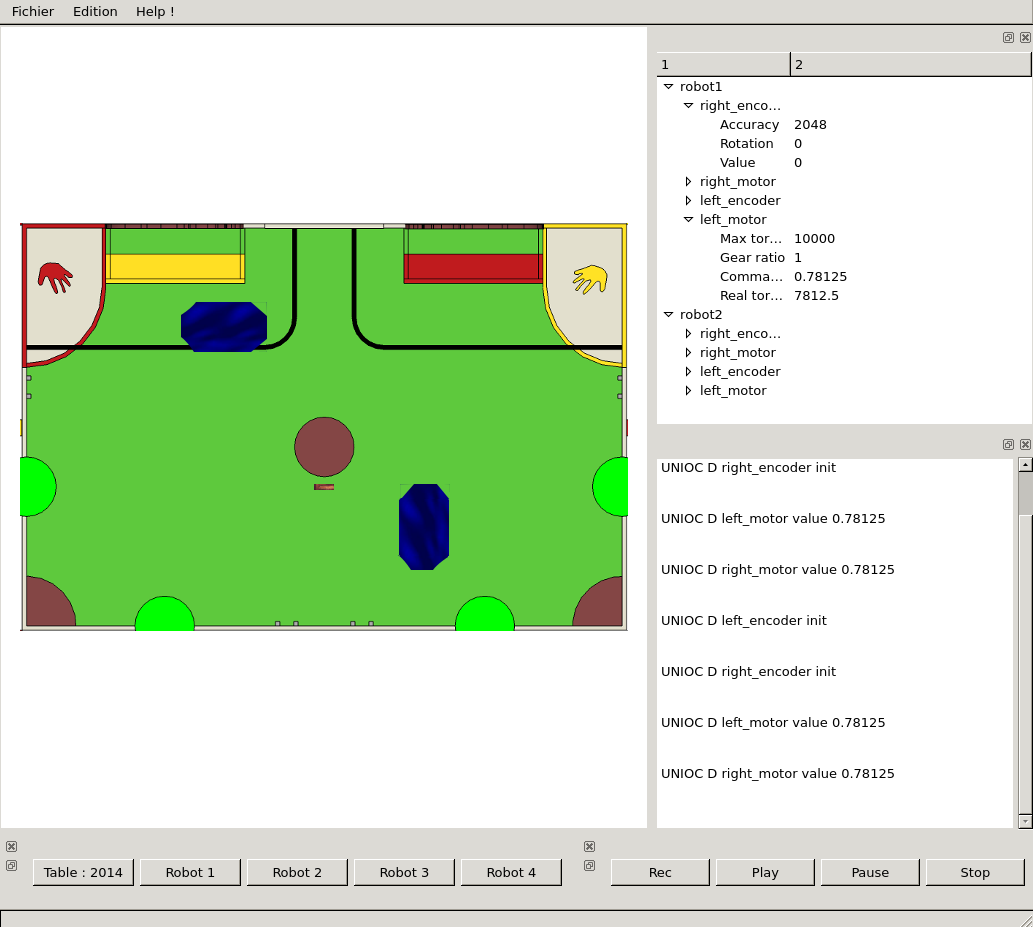
\includegraphics[width=\textwidth]{captureui.png}
\caption{Rendu final de l'interface graphique du simulateur}
\label{captureui}
\end{figure}
\clearpage

\paragraph{}
Finalement, la fenêtre d'affichage ressemble en apparence à celle présentée dans le cahier des charges (voir figure \ref{captureui}). Néanmoins, certaines fonctionnalités ne sont pas disponibles. On ne peut pas enregistrer de simulation, il n'est pas non plus possible d'enregistrer-sous une configuration de simulation. Les fonctionnalités d'insertion d'objets en cours de simulation ne sont pas implémentés.

\section{Calculateur physique}

Le moteur de simulation physique choisi est Bullet. Le cahier des charges indique qu'il est nécessaire pour le bon fonctionnement du simulateur d'utiliser un calculateur physique permettant de simuler les données à envoyer aux capteurs du robot, et de simuler un déplacement du robot proche de la réalité. Le calculateur physique est le coeur de la simulation. Outre le calcul des valeurs à renvoyer aux capteurs qui peut être fait avec une relative exactitude, la simulation d'un déplacement réaliste est le principal enjeu du calculateur physique.

\paragraph{}

L'environnement physique minimal a vu le jour en quelques jours : une table et des murs. Cependant, lors de l'arrivée des premiers tests de déplacement du robot dans cet environnement, le robot restait bloqué sans explication. Ces test reposaient sur des courbes tracées d'après les mesures faites dans le monde simulé. Nous avons donc du revoir notre méthodologie de test. Plutôt que d'afficher seulement les courbes des positions ou des vitesses, nous avons modifié une démonstration fournie avec la bibliothèque pour afficher la simulation comme le montre la figure \ref{capture3d}.

\begin{figure}[!h]
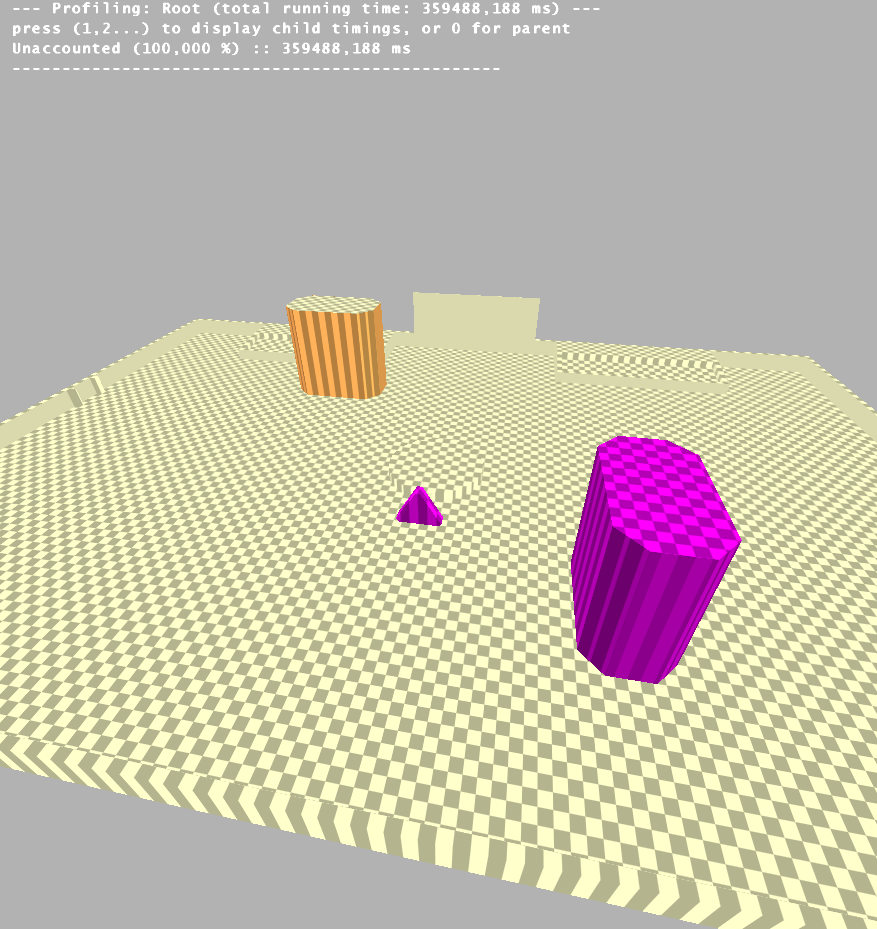
\includegraphics[width=\textwidth]{capture3d.png} 
\caption{Aperçu de la simulation 3D proposée par Bullet}
\label{capture3d}
\end{figure}
\clearpage

Il s'est avéré que les murs n'avaient pas été bien décrits. Il est difficile d'instancier un parallélépipède rectangle dans Bullet et la documentation est réellement ambiguë.


\paragraph{}

Le calculateur physique a finalement été correctement intégré au reste du simulateur, permettant de simuler les valeurs à renvoyer aux capteurs, déplacer le robot sur la table de manière réaliste. Quelques raccourcis ont été effectués, comme par exemple le calcul des valeurs à renvoyer à la balise de détection de robot adverse qui se contente de renvoyer la position relative des autres robots, sans prendre en compte le mécanisme complexe qui permet cette détection.

\paragraph{}

Le choix du moteur physique utilisé pour notre calculateur physique a été fait lors de l'élaboration du cahier des charges et c'est le moteur physique Bullet que nous avons retenu après de rapides tests. Ces tests ont nécessité de nombreuses heures d'installation et de lecture de documentation. Le manque de temps nous a donc empêché de tester d'autres calculateurs physiques. Il aurait été pourtant intéressant d'approfondir l'étude sur Bullet et d'en mener une similaire sur au moins un autre moteur physique. En effet, malgré un forum vivant, de nombreuses démos, la documentation détaillée des classes et méthodes est inexistante. Il existe seulement une documentation générale de haut niveau et une documentation html qui se contente de pointer vers des lignes de code. Le temps à investir pour comprendre l'agencement des différentes objets de Bullet n'a donc pas été négligeable. Dans l'éventualité d'un changement de calculateur nous avons fait en sorte d'interfacer au maximum l'utilisation des fonctionnalités de Bullet. Notamment pour ce qui est des modules.


\section{Modules}

Les modules ont pour but de simuler le comportement d'une partie réelle du robot, que ce soit un capteur ou un actionneur, à l'intérieur du calculateur physique. Ils doivent aussi correspondre à un device du framework et donc pouvoir recevoir des messages de ces derniers. L'objectif principal est de pouvoir imiter facilement les éléments d'origines. Ils interagissent donc directement avec le calculateur afin de lui fournir les informations nécessaires au calcul des pas de simulation et récupèrent les informations qu'ils pourraient récupérer dans la réalité. De plus, l'ajout d'un module doit pouvoir se faire facilement et sans nécessiter la recompilation du simulateur. En effet, EIRBOT évolue et il est important de pouvoir faire évoluer le simulateur en même temps.

\paragraph{}
Pour répondre à cette dernière contrainte nous avons envisagé deux solutions. La première était d'utiliser un langage interprété, le framework Qt permettant entre autres choses d'utiliser des scripts javascript. Le problème de cette méthode est l'interaction avec le reste du simulateur qui reste un peu plus coûteuse que la solution choisie. La seconde solution, et celle retenue est de créer une bibliothèque dynamique. Il n'est donc pas nécessaire de recompiler tout le simulateur lorsqu'on rajoute un module, il suffit de le compiler sous forme de bibliothèque dynamique. Le problème est que l'utilisation de bibliothèques dynamiques en C++ n'est ni simple ni portable. Ces problèmes sont simplifiés par Qt qui fournit de nombreux outils de gestion de bibliothèques dynamiques via les plugins (\texttt{QInterface}, \texttt{QPlugin}, \texttt{QPluginLoader}). Une des difficultés néanmoins rencontrées est que nous avons oublié d'inclure certaines classes à la compilation de la bibliothèque. Or, cette compilation ne lie pas les données et par conséquent ne cherche pas à savoir si les symboles des fonctions utilisées existent vraiment. Par conséquent, ce problème ne s'est révélé qu'à l'utilisation des librairies et à mis un certain temps à être résolu.

\paragraph{}
Au final, les modules ont pu être écrits sans difficultés majeures. L'écriture d'une petite API du côté du calculateur physique permet aux modules de ne pas dépendre du calculateur physique utilisé. Ces dernier remplissent leur rôle en incarnant les devices du framework Aversive++ dans la simulation physique.

\section{Coordinateur}

\paragraph{}
Le coordinateur, comme son nom l'indique, est en quelque sorte le chef d'orchestre du simulateur. Son rôle est d'assurer que chaque partie du projet communique correctement avec les autres, et reste synchronisée. Le diagramme de classe \ref{coordinatorsarchitecture} montre l'architecture que nous avons retenue du Coordinator et de ses dérivés. Il est à noter que celle-ci n'était pas la version que nous avions imaginée lors de la conception de la classe Coordinator. En effet cette classe est restée unique durant un bon mois. Mais le code devenait de plus en plus dense, presque incompréhensible. Nous avons donc choisi de "l'éclater" en utilisant le principe diviser pour régner. Ce processus est détaillé un peu plus loin.

\paragraph{}
Le coordinateur connaît donc tout le système du simulateur mais aussi celui du ou des programmes actuellement testés. Il répertorie chaque module du simulateur et chaque "device" d'Aversive++ et fait en sorte d'assurer la correspondance entre eux. Chaque élément, à son initialisation, doit donc s'identifier auprès du Coordinateur. C'est aussi ce dernier qui récupère les informations du fichier de configuration du robot et crée les éléments nécessaires. Par la suite, le Coordinateur se contente d'aiguiller les signaux Qt entre les différentes entités.

\paragraph{}

\begin{figure}[!h]
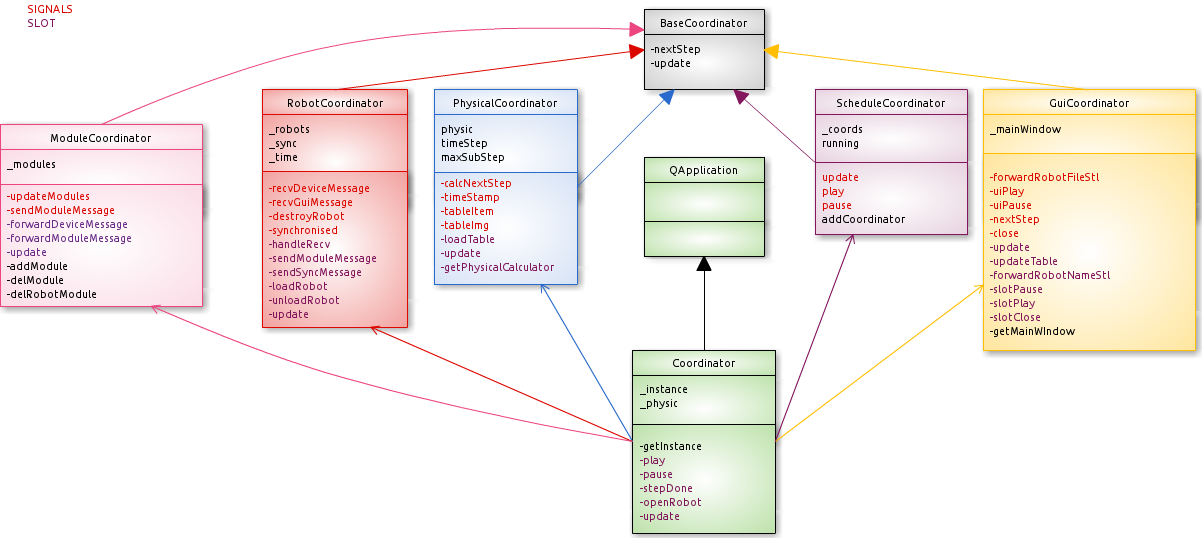
\includegraphics[scale=0.5, angle=90]{DiagClasseCoord.png}
\caption{Diagramme de classe de la construction du procédé de coordination}
\label{coordinatorsarchitecture}
\end{figure}
\clearpage

Lors du développement du Coordinateur, nous nous sommes rapidement rendu compte qu'il était surchargé de travail. En effet, il contenait de nombreux objets tels que le \texttt{MainWindow} du rendu graphique, les modules simulant capteurs et actionneurs, les robots simulés, le calculateur physique lui-même, etc. et il devait en plus ordonnancer les calculs !
Dans l'esprit de garder un code plus propre, nous avons donc décidé d'éclater cet unique coordinateur, chacun de ses collaborateurs s'occupant d'une partie spécifique du coordinateur original. Au final le \texttt{Coordinator} construit les autres coordinateurs :
\begin{itemize}
    \item Le \texttt{PhysicalCoordinator} est en charge de la gestion du calcul physique.
    \item Le \texttt{RobotCoordinator} gère la communication avec le code du robot.
    \item Le \texttt{ModuleCoordinator} s'occupe de la gestion des modules.
    \item Le \texttt{GuiCoordinator} est le coordinateur de l'interface graphique. 
    \item Le \texttt{SchedulerCoordinator} est le coordinateur spécialement dédié à l'ordonnancement des tâches et des autres coordinateurs.
\end{itemize}
Cette organisation est récapitulée par le diagramme de séquence \ref{initcoordinators} qui reprend la séquence d'initialisation des coordinateurs, et de connexion des signaux Qt. 

\paragraph{} %%\subsection{Produit final}

\begin{figure}[!h]
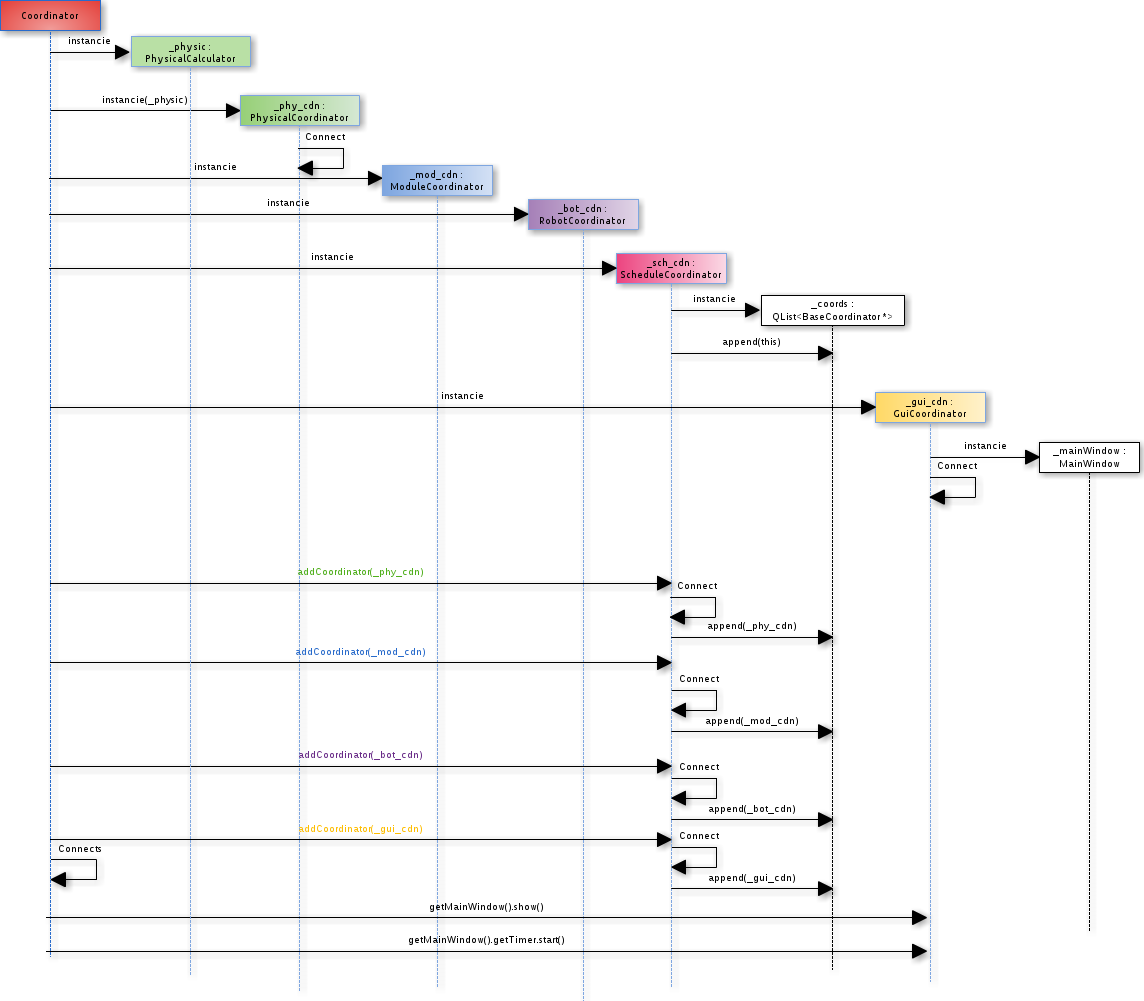
\includegraphics[scale=0.4]{DiagSeqInitCoord.png}
\caption{Diagramme de séquence sur l'initialisation des coordinateurs}
\label{initcoordinators}
\end{figure}
\clearpage


\paragraph{} Finalement, malgré la séparation imprévue du coordinateur en différents collaborateurs, le rôle initial du Coordinateur est bien respecté et l'ensemble réalise bien toutes les fonctionnalités prévues par la spécification du cahier des charges. De plus, il peut toujours gérer efficacement la synchronisation des différentes parties du simulateur et aiguiller les messages qui transitent.


\section{Communication}

La communication entre les différentes composantes du projet est primordiale pour le bon fonctionnement du simulateur. Comme il a été vu précédemment dans la partie dédiée au coordinateur, cette communication, qui doit être synchronisée, est complexe. La suite de cette partie consiste à en décrire les différents axes. Avant cela, il est important de noter que toute communication passe par le coordinateur du fait qu'il lie les signaux Qt aux Slots correspondants. La figure \ref{seqopentable} montre un exemple de l'utilisation des signaux Qt. Le principe est simple : supposons qu'il existe 3 classes A, B et C. C possède A et B. A est la classe émettrice qui possède un \texttt{signal} qu'elle \texttt{emit} dans son code. B est la classe réceptrice qui possède un Slot, qui est une méthode public dans cet exemple, avec les même arguments que le signal de A. Enfin il ne reste plus qu'à \texttt{connect(A, SIGNAL(mon_signal()), B, SLOT(mon_slot()))}.  

\paragraph{} 
Une modification importante a été effectuée concernant la communication. Alors que le cahier des charges mentionnait l'utilisation de \texttt{socket} de communication entre le simulateur et le ou les exécutables robots. Il s'est avéré bien plus simple et plus efficace de ne communiquer qu'à partir de manipulation sur l'entrée et sortie standard de ces exécutables robots.

\begin{figure}[!h]
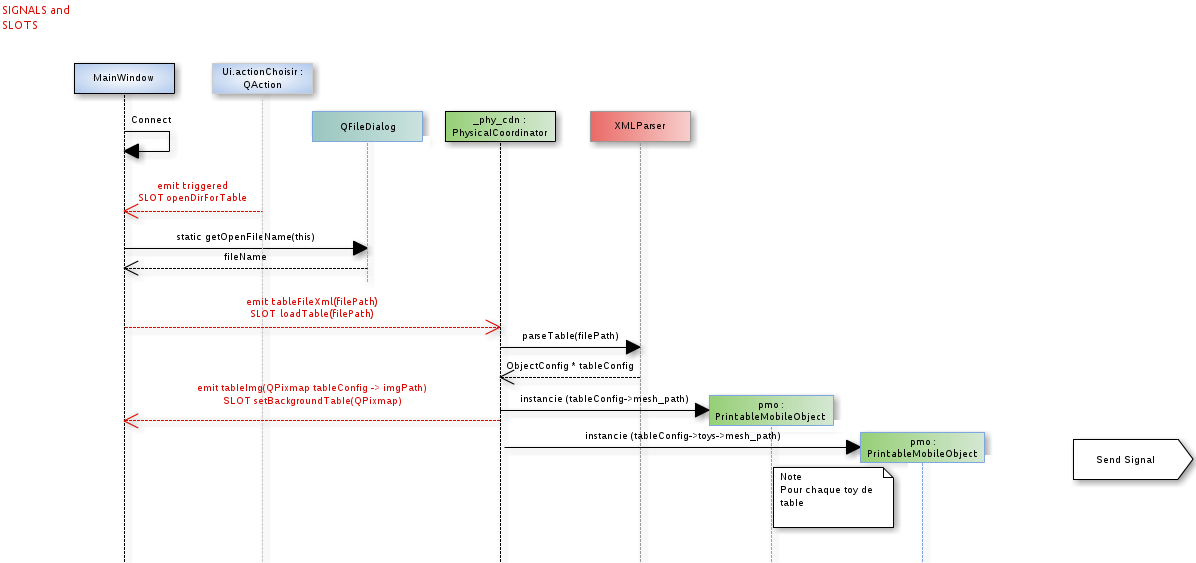
\includegraphics[scale=0.5]{DiagSeqOpenTable.png}
\caption{Diagramme de séquence : choix d'une table par l'utilisateur}
\label{seqopentable}
\end{figure}
\clearpage


\subsection{Calculateur physique et interface graphique}
\label{calcgui}
La communication entre le calculateur physique et l'interface graphique est celle qui permet à l'utilisateur de voir en temps réel l'état de la table. Elle permet à l'interface graphique de rafraîchir régulièrement les informations qu'elle possède à partir des données calculées.

\paragraph{}
Cette partie du projet soulève de nombreuses difficultés. En particuliers, la configuration antique des ordinateurs du client soulèvent des problèmes d'optimisation de la performance, ce qui est un enjeu crucial dans la simulation physique. De manière à fournir un affichage fluide nous avons utilisé le système de signaux de la librairie Qt. Cela résout donc le problème de fréquence d'affichage mais pas celui de l'affichage des robots et autre objets sur la table. La première idée a été de créer une liste pour tous les objets à afficher et de la parcourir à chaque pas de simulation. Mais cette méthode était trop peu modulaire. La solution finale à donc été de créer une classe PMO (\texttt{printable mobile\footnote{La Table est un PMO sans être mobile, mais nous avons estimé que ce détail n'est pas crucial} object}). Cette classe possède les méthodes nécessaires à l'affichage de chaque objet dans la simulation 2D. Tout élément devant être affiché hérite donc de cette classe. La position des objets est ainsi accessible par la méthode \texttt{getPosition} qui utilise directement les fonctionnalités du calculateur physique pour obtenir la position du-dit objet. Donc, plutôt que d'avoir une liste pour chaque type d'objet à afficher il n'y a qu'une liste de PMO à gérer et ses éléments s'y ajoutent d'eux même à leur initialisation.

\paragraph{}
Les PMO ne sont pas des objets Qt et cela nous a posé un problème au cours de l'intégration du projet. En effet Qt crée de nouveaux objets pour générer l'affichage. Il était alors difficile de retrouver quels objets Qt correspondaient à tel ou tel PMO. L'architecture générale a donc dû être modifiée pour relier l'affichage de Qt aux PMO du calculateur physique. Les PMO ont donc un objet \texttt{QGraphicsView}. Enfin le coordinateur rajoute les éléments de la liste des PMO dans l'interface graphique. Afin d'optimiser l'espace mémoire utilisé par le rendu graphique les images (PixMaps) on été rangées dans un ensemble afin d'éviter les doublons et vérifie que l'image n'est plus utilisée avant de la supprimer.

\subsection{Communication du Device au Module}

Un device est un objet (au sens de la Programmation Orientée Objets) qui représente une entrée/sortie du point de vue du code robot. Sur un robot réel, cela peut correspondre à un capteur, un actionneur ou un canal de communication avec un autre système. Dans SASIAE, un device est connecté à un Module, qui se charge de lui envoyer des données, ou de faire des action sur le calculateur physique.
Ainsi, à un module doit correspondre un et un seul device.

\paragraph{}
Les devices et modules sont identifiés par des chaînes de caractères qui représentent leur nom. Ce nom est donc utilisé pour acheminer les messages au bon device ( resp. module). Il est défini par l'utilisateur dans le fichier décrivant le robot pour les modules, et dans le code source à la construction des objets pour les devices.
Un problème peut survenir lorsque plusieurs robots dans la simulation ont des noms de device/module identiques. Il faut donc pouvoir acheminer les messages aux modules et devices qui correspondent au bon robot. Pour cela les robots sont identifiés par un nom représenté par une chaîne de caractères.

Les entités qui s'occupent de l'acheminement des messages sont :
\begin{itemize}
\item Device (Aversive++)
\item ClientThread (Aversive++)
\item RobotCoordinator (SASIAE)
\item ModuleCoordinator (SASIAE)
\item Module (SASIAE)
\end{itemize}
Ces objets se transmettent des messages sous forme de chaîne de caractères. La transmission a été pensée comme un modèle en couches comme le modèle OSI ou le modèle TCP/IP. En effet, à chaque transmission, des informations de routage sont ajoutées au message original pour le transmettre au correspondant.
Le diagramme \ref{commoduledevice} représente le cheminement des messages entre les différentes entités.

\begin{figure}[!h]
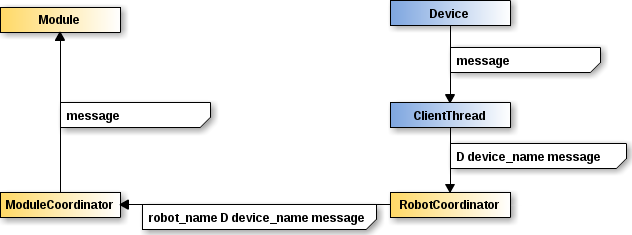
\includegraphics[scale=0.5]{DiagComModuleDevice}
\caption{Diagramme présentant le cheminement d'un message d'un device vers un module.}
\label{commoduledevice}
\end{figure}
\clearpage

\paragraph{}

Le protocole de communication entre les modules et les devices est laissé libre (en annexe à la section \ref{convcomm}). Cependant, une convention de messages standards a été définie pour guider à la création de nouveaux modules/devices.
Une fois le message transmis au \texttt{ClientThread} ou au \texttt{ModuleCoordinator}, ce dernier est préfixé par le caractère "D" suivit d'un espace et du nom de module/device. Le \texttt{ClientThread} envoie donc le message au \texttt{RobotCoordinator}.
Le message transmis entre \texttt{RobotCoordinator} et \texttt{ModuleCoordinator} est alors préfixé du nom du robot correspondant.

Un autre problème fut rencontré lorsque plusieurs messages étaient envoyés simultanément. Le coordinateur ne recevait qu'un seul signal alors que plusieurs messages étaient en attente. Le bug fut corrigé en forçant le coordinateur à lire tous les messages disponibles dès la réception d'un signal.

\paragraph{}
Dans le cahier des charges, cet aspect de la communication n'avait pas été abordé avec précision, ce qui explique que de nombreuses modifications ont dû être apportées au fil de l'écriture du code, pour s'adapter aux contraintes qui apparaissaient. Toute fois, ces différences sont transparentes pour les modules et devices qui communiquent tel qu'il était prévu à l'origine.

\section{Langage de description}

Le cahier des charges prévoyait de créer un fichier de description de la table et des robots. Fourni par l'utilisateur il permettra d'adapter le simulateur à la table de l'année et à la configuration interne des robots. La description détaillée des fichiers de configuration est située en annexe du cahier des charges. Ce langage à été prévu en XML afin d'être compréhensible par un utilisateur et directement éditable. Il a donc fallu créer une interface permettant d'extraire les données de ce document afin que le simulateur puisse les exploiter. Et ainsi créer un jeu de structures de données reprenant l'arborescence des fichiers XML. En avançant dans l'intégration des différents éléments nous nous sommes aperçu qu'il manquait certains éléments dans la description du cahier des charges, que nous avons par conséquent rajouté, comme par exemple le poids total du robot, un fichier image pour afficher la table dans le rendu graphique... Pour ce qui est des tests, nous avons simplement testé les différents cas d'utilisation de la fonction d'extraction de données du fichier. Des exemples de fichier de description sont donnés en annexe à la section \ref{descXML}.






\chapter{Bilan}
\section{Avancement du projet}

Comme nous l'avons rapidement exposé lors de la description de la stratégie de découpage du temps, nous n'avons pu aller jusqu'au cinquième et dernier livrable. Seul le 4ème livrable a été fini. Cela signifie que nous sommes en mesure de charger des configurations de tables et de robots, de les afficher dans l'interface graphique. La plupart des modules et devices ont été écrits, et seuls ceux qui sont très rarement utilisés par le client EIRBOT ont été mis de côté.
Nous pouvons également rajouter dynamiquement des modules sans recompiler l'ensemble du projet.

\paragraph{}
Très peu de codes robot ont pu être testés jusqu'à présent, mais le client est satisfait de la version produite par l'équipe de PFA.

\paragraph{}
La trajectoire est relativement conforme à celle observée dans la réalité, même si le robot simulé sur-réagit parfois lors de chocs contre le bord de la table. On observe en effet de temps en temps que le robot est à la limite de basculer d'avant en arrière et peut mettre du temps à retrouver son équilibre.

\section{Retour d'expérience}

Ce projet a été très enrichissant. Pour le mener à bout, il a fallu prendre en main des librairies volumineuses, se plonger dans leurs documentations et lutter contre leurs problèmes de compatibilité. Ce projet est aussi le premier véritable projet que nous menons puisqu'il est destiné à un client réel. Le fait que ce projet soit porté par des élèves de l'ENSEIRB-MATMECA ne retire rien à l'importance et à la pression du client puisque nous le côtoyons tous les jours. Finalement, ce projet nous a permis de nous rendre compte de nos capacités à travailler en groupe à des fins pédagogiques et professionnelles. Cela nous a permis de partager nos connaissances et de les appliquer dans des problèmes classiques tels que l'ordonnancement de processus, l'optimisation d'un affichage ou encore la création d'un langage de configuration.

\paragraph{}
L'organisation du travail au sein du groupe a représenté une difficulté importante. Il a fallu gérer les rythmes de chacun. Le travail de groupe est un échafaudage constant basé sur des dissensions, des ententes et des concessions. Un autre problème est de gérer les capacités de chacun. En effet, notre groupe était constitué de membres ayant des maîtrises et des savoirs très différents et certains très avancés. Des discussions se sont souvent retrouvées bloquée plus par entêtement que par réelle difficulté. De plus, il y a eu des difficultés à adapter le rythme du projet au rythme de notre vie scolaire ce qui a donné des périodes de relâchement pénalisantes dans les derniers jours. Comme nous l'avons présenté en début de ce document, nous avons essayé différentes méthodes pour gérer notre projet. Au final, ce sont les réunions hebdomadaires, tous ensemble, qui on été les plus productives. 

\chapter{Annexe}

\section{Comment utiliser SASIAE}
SASIAE ne nécessite pour fonctionner que des bibliothèques dynamiques de Qt5, celles-ci sont utilisées par le simulateur pour gérer l'affichage ainsi que de nombreuses communications entre les entités du simulateur. Cependant, à moins d'être en possession d'un code robot déjà exécutable, il est nécessaire de pouvoir compiler le code écrit afin de le tester dans le simulateur. Le compilateur avr-gcc peut également être installé pour obtenir un code exécutable sur une architecture AVR, utilisée par les robots d'Eirbot. De cette manière, il devient possible de confronter la simulation à la réalité d'un robot roulant sur la table.

\paragraph{}
Pour obtenir une simulation la plus proche possible de la réalité, il est conseillé de fournir au programme des fichiers STL (format standard de représentation 3D) représentant la table et les robots le plus fidèlement possible. La table étant commune à toutes les équipes qui participent à la coupe de France de robotique, sa représentation STL peut être trouvée sur le web. Néanmoins celle du robot est propre à chaque équipe.

Cependant le fichier STL ne suffit pas pour décrire la table ou les robots. Pour la table, les éléments mobiles doivent être rajouté dans le fichier XML de description. Pour les robots, les blocs particuliers tels que les encodeurs, les roues motrices, ou les capteurs de distance doivent également être rajoutés dans le fichier XML.

Pour finir, il faut indiquer pour chaque robot où se trouve son code. Il s'agit donc encore une fois de renseigner cette information dans le fichier XML.

\paragraph{}
Une fois que le simulateur est en possession de toutes les informations relatives au(x) robot(s) et à la table, celui-ci est en mesure d'afficher en temps réel le déplacement des robots sur la table. À la droite de l'écran se situe un cadre qui indique en temps réel les valeurs renvoyées par les capteurs des robots ainsi que celles assignées aux actionneurs. Une première étape pour faciliter le débuggage de votre code !

\newpage
\section{Tests}
\label{lestests}
\subsection{Client Thread et Devices}

Le \texttt{client thread} est testé à l'aide d'un coordinateur fictif. On emploie donc on système de serveur/client. Le client est un code robot vide avec un faux device qui répond aux sollicitations du serveur qui vérifie leur leur cohérence. De même, le test des devices fonctionnent sur le principe client/serveur ou le serveur est un coordinateur fictif qui soit envoie des données au device et on teste la bonne utilisation de ces dernières, soit on envoie des données au serveur et on vérifie la cohérence des échanges, soit les deux. De plus, les test sont formatés de manière à pouvoir tester rapidement tous les device et ainsi vérifier la non-régression du framework.
 
\subsection{Scheduler}

Le scheduler aussi est testé sur le système client/serveur puisque qu'il est synchronisé avec le simulateur. On fournit donc une fausses liste tâches avec diverses priorités et diverses périodicités. Les tâches envoient des messages et on vérifie que les dates de réception de ces messages sont bien les dates prévues.


\subsection{Interface Graphique}

L'interface graphique est sans nul doute la plus difficile à tester, puisque l'on ne peut pas tout tester à la main et qu'il est compliqué d'automatiser les testes. Cependant on a testé les signaux en les redirigeant de manière à constater leur fonctionnement et de même pour leur chaînage.

\subsection{Modules}

Les modules interagissent avec deux choses, le coordinateur et le coordinateur physique. Ils sont donc un peu plus difficiles à tester. De plus, comme il est difficile de faire un faux simulateur physique, nous les avons testés dans des situations de simulation maîtrisée et nous avons vérifié la cohérence des messages générés en les stimulants à la main si nécessaire par un serveur prenant les messages d'entrée en ligne de commande.

\subsection{Calculateur physique}

Enfin, nous avons testés le fonctionnement de notre utilisation du calculateur physique. Comme il est précisé dans la partie dédiée plus haut, nous avons d'abord extrait les vecteurs positions et vitesse des robots afin de les représenter par des courbes. Les informations ainsi obtenues étant trop difficile à exploiter, nous avons ensuite affiché directement une vue 3D de la simulation pour voir ce qui se passait.

\section{Protocoles et format XML}
\subsection{Protocoles de comunication}
\label{convcomm}
\begin{verbatim}

From SASIAE to Robot:
     "T xxx yyy\n" : synchronization command, xxx must be microseconds since the
simulation started, yyy is the amount of iteration of robotLoop to execute
     "B\n" : begin the match
     "D xxx yyy\n" : send yyy message to xxx named device
     "S\n" : stop the simulation

From Robot to SASIAE:
     "D xxx yyy\n" : send yyy message to xxx named
     "M t xxx\n" : t among I(nfo), W(arning), E(rror) or D(ebug), xxx is the message
     "T" : notify the coordinator that the robot has finished executing its step

For "D xxx yyy\n" messages, yyy must be:
    - "init v v v ..."
    - "value v"
    - "ivalues i:v i:v i:v ..."
    - "values v v v ..."

If v is a string, it must be surrounded by " (double-quotes), double-quotes and
"\" (backslashes) must be escaped with a "\".
String shouldn't contain new-line character (ASCII code 10) by any means.

\end{verbatim}
\subsection{Exemples de fichiers de description}
\label{descXML}

\begin{lstlisting}[caption=Exemple de description d'un robot, label=desctable]
<robot weight="20">
    <mesh src="../ressources/stl/robot1.stl" scale="0.1"/>
    <img src="../ressources/img/robot.png"/>
        <microcontrollers>
            <microcontroller name="UNIOC">
                <modules>
                    <module name="roue droite" type="MotorWheel">
                        <location X="10" Y="-2" Z="10" alpha="0" beta="0" gamma="0"/>
                        <parameters>
                            <parameter name="wheel_radius" type="float" value="3"/>
                            <parameter name="max_torque" type="double" value="1000."/>
                            <parameter name="gear_ratio" type="double" value="1."/>
                        </parameters>
                    </module>
                    <module name="encodeur droite" type="Encoder">
                        <location X="11" Y="-2" Z="10" alpha="0" beta="0" gamma="0"/>
                        <parameters>
                            <parameter name="wheel_radius" type="float" value="3"/>
                            <parameter name="accuracy" type="int" value="2048"/>
                        </parameters>
                    </module>
                </modules>
            </microcontroller>
    </microcontrollers>
</robot>
\end{lstlisting}

\begin{lstlisting}[caption=Exemple de descritption d'une table, label=desctable]
<table>
    <mesh src="../ressources/stl/table_static_2014_2.stl" xOffset="-100" zOffset="100" />
    <img src="../ressources/img/table_2014_rognee.png"/>
        <toys>
        <toy name="triangle1" weight="170" >
            <location X="10" Y="10" Z="10" alpha="0" beta="0" gamma="0"/>
                <mesh src="../ressources/stl/feutext.stl" scale="0.1"/>
                <img src="../ressources/img/feu.png"/>
        </toy>
    </toys>
</table>
\end{lstlisting}
%\section{Cahier des charges}

\end{document}